\section{Data Preprocessing and Preparation}
\label{sec:preprocessing}

Fig.~\ref{fig:pipeline} shows the pipeline from raw annotations to training batches. Each step is a command in the project repository, and the steps run in the order given here.

\begin{figure}[tbp]
  \centering
  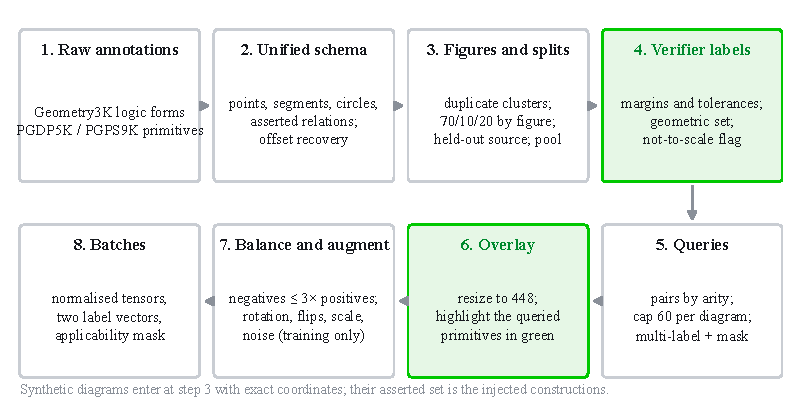
\includegraphics[width=\textwidth]{fig_pipeline}
  \caption{The data pipeline. Green steps are the two that distinguish this study: the verifier that produces the geometric labels, and the overlay that turns a query into an image.}
  \label{fig:pipeline}
\end{figure}

\subsection{Unified schema and loaders}

One loader per source converts the raw annotation into a single \texttt{Diagram} record: image path and size; points as name $\to$ pixel coordinates (origin top-left); segments as pairs of point names; lines as collinear point groups; circles as centre, radius and the points on them; and the asserted relations with their type and arguments. For Geometry3K, whose positions carry a per-diagram translation, the loader recovers the offset by matching the positions to the red dots in the point-annotated image (all points matched in 2,985 of 3,001 diagrams with points; the remainder are flagged). Geometry3K stores no numeric radius, so the loader uses the median distance from the centre to its annotated on-circle points. Every relation name is mapped to one of the six target relations by a fixed table (for example \texttt{PointLiesOnCircle} $\to$ \rel{on\_circle}; a right-angle symbol $\to$ \rel{perpendicular}), so that all sources share one definition. A sanity check confirms that annotated points fall inside the image (\pctGeometryPointsOutside\% of Geometry3K points do not, after offset recovery; none in the other sources).

\subsection{Figure clustering and splits}

Because the same figure recurs across problems and across datasets, the unit of splitting is the \emph{figure}, a cluster of duplicate images. Candidates are found by a 64-bit difference hash within a small Hamming distance and confirmed by near-identical pixels at low resolution or by the overlap of their ink together with agreement of the labelled point names; low-resolution similarity alone was found to match different simple triangles and is not enough. The \nGeometryFigures{} Geometry3K figures are re-split \splitPctTrain/\splitPctVal/\splitPctTest{} with a fixed seed, stratified by whether the figure contains a circle, into \nFiguresTrain{} / \nFiguresVal{} / \nFiguresTest{} figures. Where PGDP5K re-annotated a figure, its pixel-accurate annotation replaces Geometry3K's; otherwise Geometry3K's is kept. The held-out source is the \nHeldoutFigures{} PGDP5K test figures that have no Geometry3K copy, and the self-training pool is the \nPoolFigures{} PGPS9K figures that appear in no validation or test set (only the ones outside the training split are pseudo-labelled). A test asserts that no diagram and no figure appears in two units.

\subsection{Geometric labelling by the verifier}
\label{sec:verifier}

The verifier decides every relation from coordinates in double precision. Each check returns the raw \emph{margin}, a scale-free quantity that measures how far the primitives are from satisfying the relation, and the decision is the margin compared with a fixed tolerance (Table~\ref{tab:verifier}). Relative tolerances make the checks independent of image size; for \rel{collinear} the distance is normalised by the \emph{diagram scale}, the diagonal of the bounding box of all points. Two refinements came from the gold-set audit below: a segment with both endpoints on the circle is a chord, not a tangent, and the tangency point may sit at a segment's end; and two coincident lines are not counted as parallel.

\begin{table}[tbp]
  \centering\small
  \caption{Relation checks. $\theta$ is the angle between two segments, $|s|$ a segment length, $c$ and $r$ a circle's centre and radius, $d(\cdot)$ a point-to-line distance, $D$ the diagram scale. A query is positive when its margin is at most the tolerance.}
  \label{tab:verifier}
  \begin{tabular}{@{}l l l l@{}}
    \toprule
    Relation & Margin & Tolerance & Origin of the value \\
    \midrule
    \rel{parallel}      & $|\sin\theta|$                              & $\sin(\tolParallelDeg^\circ)$       & valley at \valleyParallelDeg$^\circ$, widened after gold round 1 \\
    \rel{perpendicular} & $|\cos\theta|$                              & $\sin(\tolPerpendicularDeg^\circ)$  & valley at \valleyPerpendicularDeg$^\circ$, widened after gold round 1 \\
    \rel{equal\_length} & $\bigl||s_1|-|s_2|\bigr| / \max(|s_1|,|s_2|)$ & \tolEqualLengthPct\%               & knee at \kneeEqualLengthPct\%, widened after gold round 1 \\
    \rel{on\_circle}    & $\bigl||p-c|-r\bigr| / r$                   & \tolOnCirclePct\%                   & density valley \\
    \rel{tangent}       & $|d(c, s)-r| / r$, foot on $s$, not a chord & \tolTangentPct\%                    & equals \rel{on\_circle} (no asserted tangents) \\
    \rel{collinear}     & $|(b-a)\times(p-a)| / (|b-a|\,D)$           & \tolCollinearPct\% of $D$           & density valley \\
    \bottomrule
  \end{tabular}
\end{table}

\paragraph{Calibration.} For each relation, the margin is computed for every candidate query in the training split and split by whether the query is asserted (Fig.~\ref{fig:tolerance}). The initial tolerance is the valley between the two modes of the smoothed log-margin density, or, where there is no valley (\rel{equal\_length}), the knee of the asserted cumulative distribution.

\begin{figure}[tbp]
  \centering
  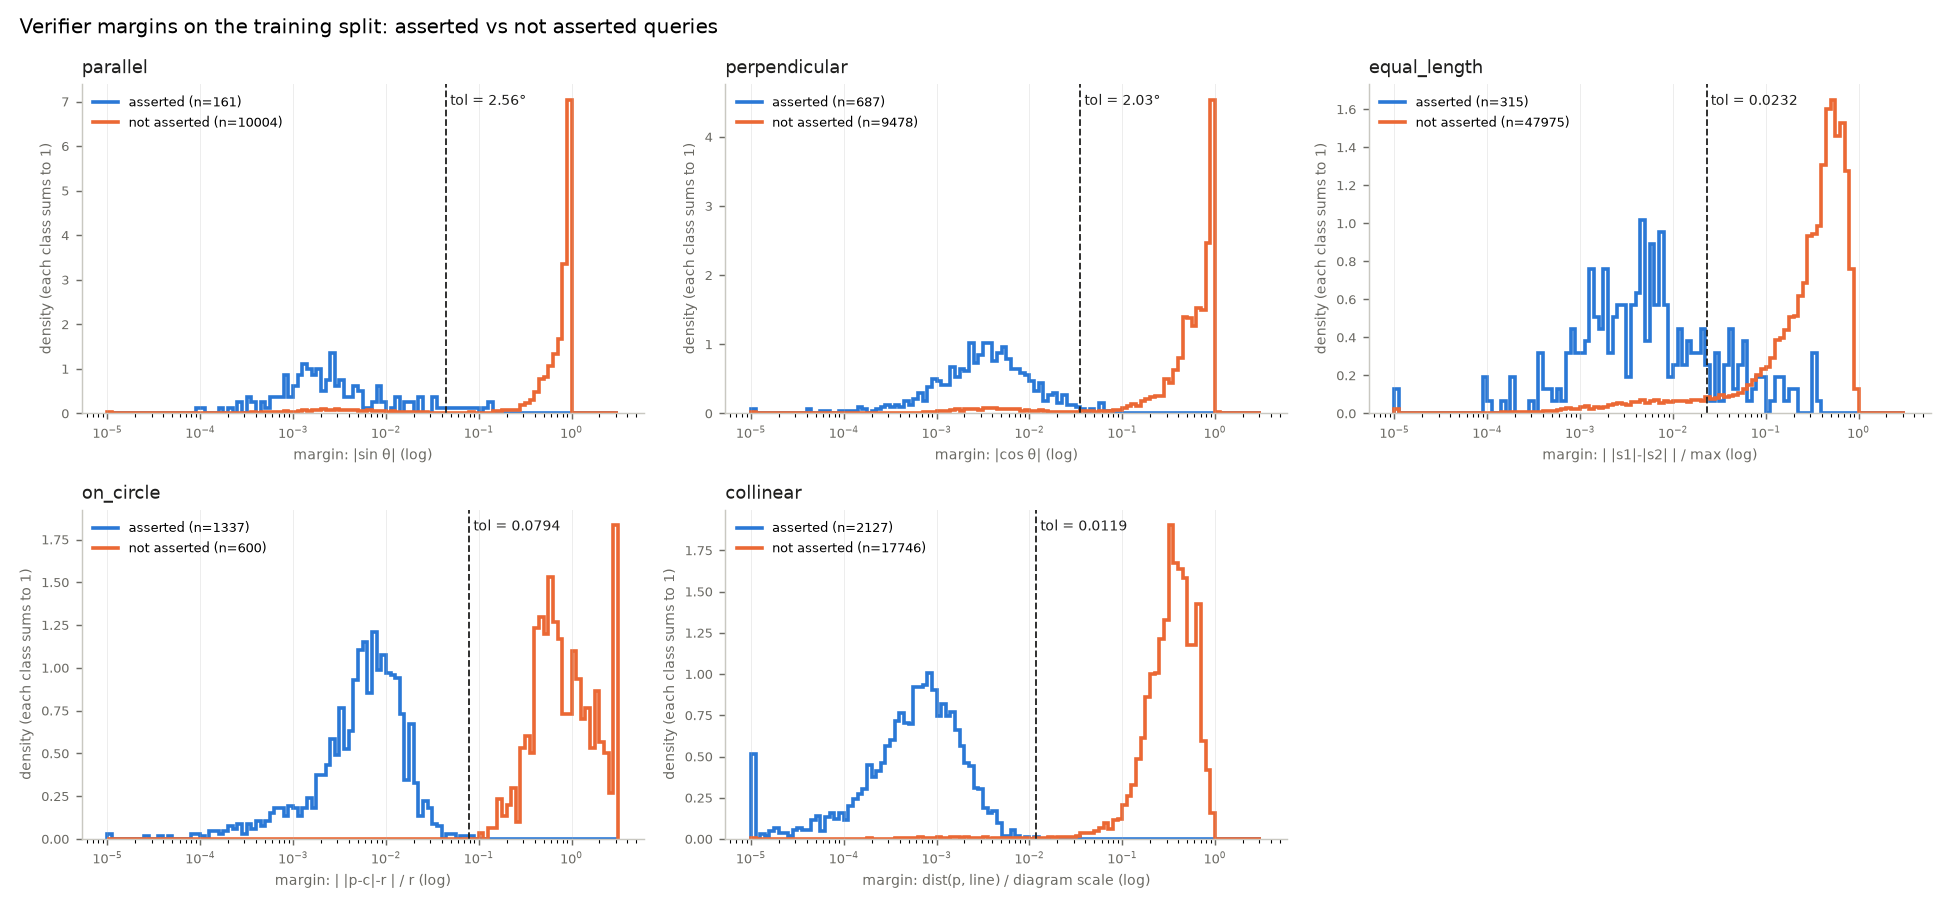
\includegraphics[width=\textwidth]{tolerance_all}
  \caption{Margin distributions on the training split, asserted queries against the rest, with the calibrated thresholds. The annotation and the drawing agree for most relations; the overlap for \rel{equal\_length} is the reason its tolerance was set by a human audit rather than by the histogram.}
  \label{fig:tolerance}
\end{figure}

\paragraph{Gold-set validation.} Because the verifier is the measuring instrument of the whole study, its agreement with a human reading of the diagram is checked on a gold set labelled by eye, without access to the annotation, with a pre-registered ceiling of \goldCeilingPct\% for both the false-positive and the false-negative rate. Round~1 (\nGoldRoundOne{} queries, enriched near the tolerances) failed the gate (FP \pctGoldRoundOneFP\%, FN \pctGoldRoundOneFN\%): the eye accepts more than the histogram valleys, so the angle tolerances were widened to \tolParallelDeg$^\circ$ and the length tolerance to \tolEqualLengthPct\%, within the range consistent with every round-1 label. Because round~1 informed the revision, the gate is decided on a fresh round~2 (\nGoldRoundTwo{} new queries plus a blind re-check of round-1 disagreements mixed with as many agreements), scored with population weights that undo the near-tolerance oversampling. The raw round-2 rates were FP \pctGoldRoundTwoWeightedFP\% and FN \pctGoldRoundTwoWeightedFN\%, the latter driven by \nGoldAdjudicated{} items that the labeller, on re-inspection, confirmed as slips (a radius labelled tangent; sides 24\% apart labelled equal); they are recorded in an adjudication file with the raw labels untouched. The adjudicated weighted rates are FP \pctGoldRoundTwoAdjFP\% and FN \pctGoldRoundTwoAdjFN\%, which passes the gate; the unweighted stress rates are reported alongside (FP \pctGoldRoundTwoAdjStressFP\%, FN \pctGoldRoundTwoAdjStressFN\%).

\paragraph{Labels and flags.} With the tolerances fixed, the verifier enumerates every candidate query of every diagram and writes the \emph{geometric} relation set with its margins, next to the \emph{asserted} set. A diagram is flagged \emph{not to scale} when any asserted relation fails its check by a large margin (more than \ntsAngleDeg$^\circ$ for angles or \ntsLengthPct\% for lengths); flagged diagrams stay in the data and are evaluated as a separate category. The flag fires on \pctNtsGeometryFigures\% of the curated Geometry3K figures, \pctNtsPgdp5k\% of PGDP5K and \pctNtsPgps9k\% of PGPS9K.

\subsection{Query enumeration and labels}

Candidate queries are enumerated per diagram by arity: all segment pairs, all point--circle pairs, all segment--circle pairs, and all point--segment triples, excluding nested sub-segments of one drawn line. To bound the dataset, at most \queryCap{} queries per diagram are kept: in the training unit every positive is kept and negatives fill the remainder; in evaluation units the sample is uniform, so the natural ratio of positives to negatives is preserved. Each query carries two six-dimensional label vectors (geometric and asserted) and the applicability mask of its kind. The resulting units hold \nTrainQueries{} training queries, \nQueriesGeometryTest{} in-distribution test queries, \nQueriesPgdpHeldout{} held-out-source queries and \nQueriesSynthExtrap{} extrapolation queries, of which \extrapEvalCap{} evenly spaced ones are evaluated.

\subsection{Overlay rendering and normalisation}

A query becomes an image by drawing the queried primitives on the diagram in a fixed highlight colour, RGB (\overlayRGB), \overlayWidthPx{} px wide with a semi-transparent halo of \overlayHaloPx{} px; a point is drawn as a filled marker and a circle is traced. Everything else is left unchanged, and a unit test asserts that no pixel outside the highlighted primitives is altered. The colour was chosen by measurement: in \nColourImages{} sampled real diagrams, red, orange and cyan ink occur in \pctColourRed\%, 68\% and 14\% of images respectively and blue in \pctColourBlue\%, whereas no image (\nColourNearHighlight{} of \nColourImages) contains a colour within distance 80 of the highlight, so the highlight cannot be confused with ink. The image is first resized so that its long side is \inputLongSide{} px with the aspect ratio preserved, then the overlay is drawn (so the highlight has the same width in every input), then the image is padded with white to a multiple of \inputPadMultiple{} px, the backbone's patch size, and normalised with the backbone's mean and standard deviation. Overlays are cached to disk as PNG, keyed by diagram and query. The dataset object returns, per query, the normalised tensor, both label vectors, the mask and metadata; batches of \ftBatch{} are padded with normalised white to the largest image in the batch.

\subsection{Negative balancing and class weights}

Negatives dominate the natural query distribution. For training only, the all-negative queries of each query kind are downsampled to at most \noneRatio$\times$ the number of positive queries of that kind, so that the head does not collapse to \rel{none}. In addition the loss weights each relation's positives by the ratio of applicable negatives to positives in the training split, capped at \posWeightCap{}. Evaluation units keep the natural ratio.

\subsection{Relation-preserving augmentation}

Training images are augmented after the overlay, so the highlight transforms with the diagram: rotation by up to $\pm\augRotationDeg^\circ$, horizontal and vertical flips, scaling of the ink box by \augScaleMin--\augScaleMax{} (as a crop and resize capped at the input size, so nothing is cut), line thickening by a $3\times3$ minimum filter with probability \augThickenProb, Gaussian noise with standard deviation up to \augNoiseStdMax, JPEG re-encoding at quality \augJpegMin--\augJpegMax, and contrast change by \augContrastMin--\augContrastMax. Shear and perspective are excluded because they break parallelism and length equality, and therefore the labels.

\subsection{Synthetic diagram generation}

The generator samples \synthPointsMin--\synthPointsMax{} points on a \synthCanvasPx{} px canvas with a minimum separation of \synthMinSeparationPx{} px, \synthSegmentsMin--\synthSegmentsMax{} segments and up to \synthCirclesMax{} circles. Each construction step, with probability \synthInjectRate, injects a relation exactly (a segment parallel or perpendicular to another, a segment of equal length, a point on a segment or on a circle, a tangent at a circle point; \rel{tangent} is weighted double because real data has no positives), otherwise it adds a random point or segment. The injected constructions form the synthetic \emph{asserted} set and are drawn as textbook marks. The diagram is then rotated by up to \synthRotationDeg$^\circ$ and every coordinate is jittered by Gaussian noise of \synthJitterPx{} px, so that the \emph{geometric} truth is decided by the verifier rather than by the construction, exactly as for real data. Rendering varies line width, font, label offset and, with some probability, scan noise and JPEG artefacts (Fig.~\ref{fig:synthetic}). A verification pass confirms that injected relations pass their checks in at least \synthInjectedPassMinPct\% of cases while random candidates pass in at most \synthRandomPassMaxPct\% (\synthRandomPassEqualLengthPct\% for \rel{equal\_length}, whose chance rate is higher). Every diagram is a pure function of the seed and its index, so the pools regenerate bit-for-bit on any machine. The extrapolation pool uses \synthExtrapPointsMin--\synthExtrapPointsMax{} points; the unlabelled pool's annotation is sealed with a SHA-256 digest before any experiment and opened only for post-hoc analysis.

\begin{figure}[tbp]
  \centering
  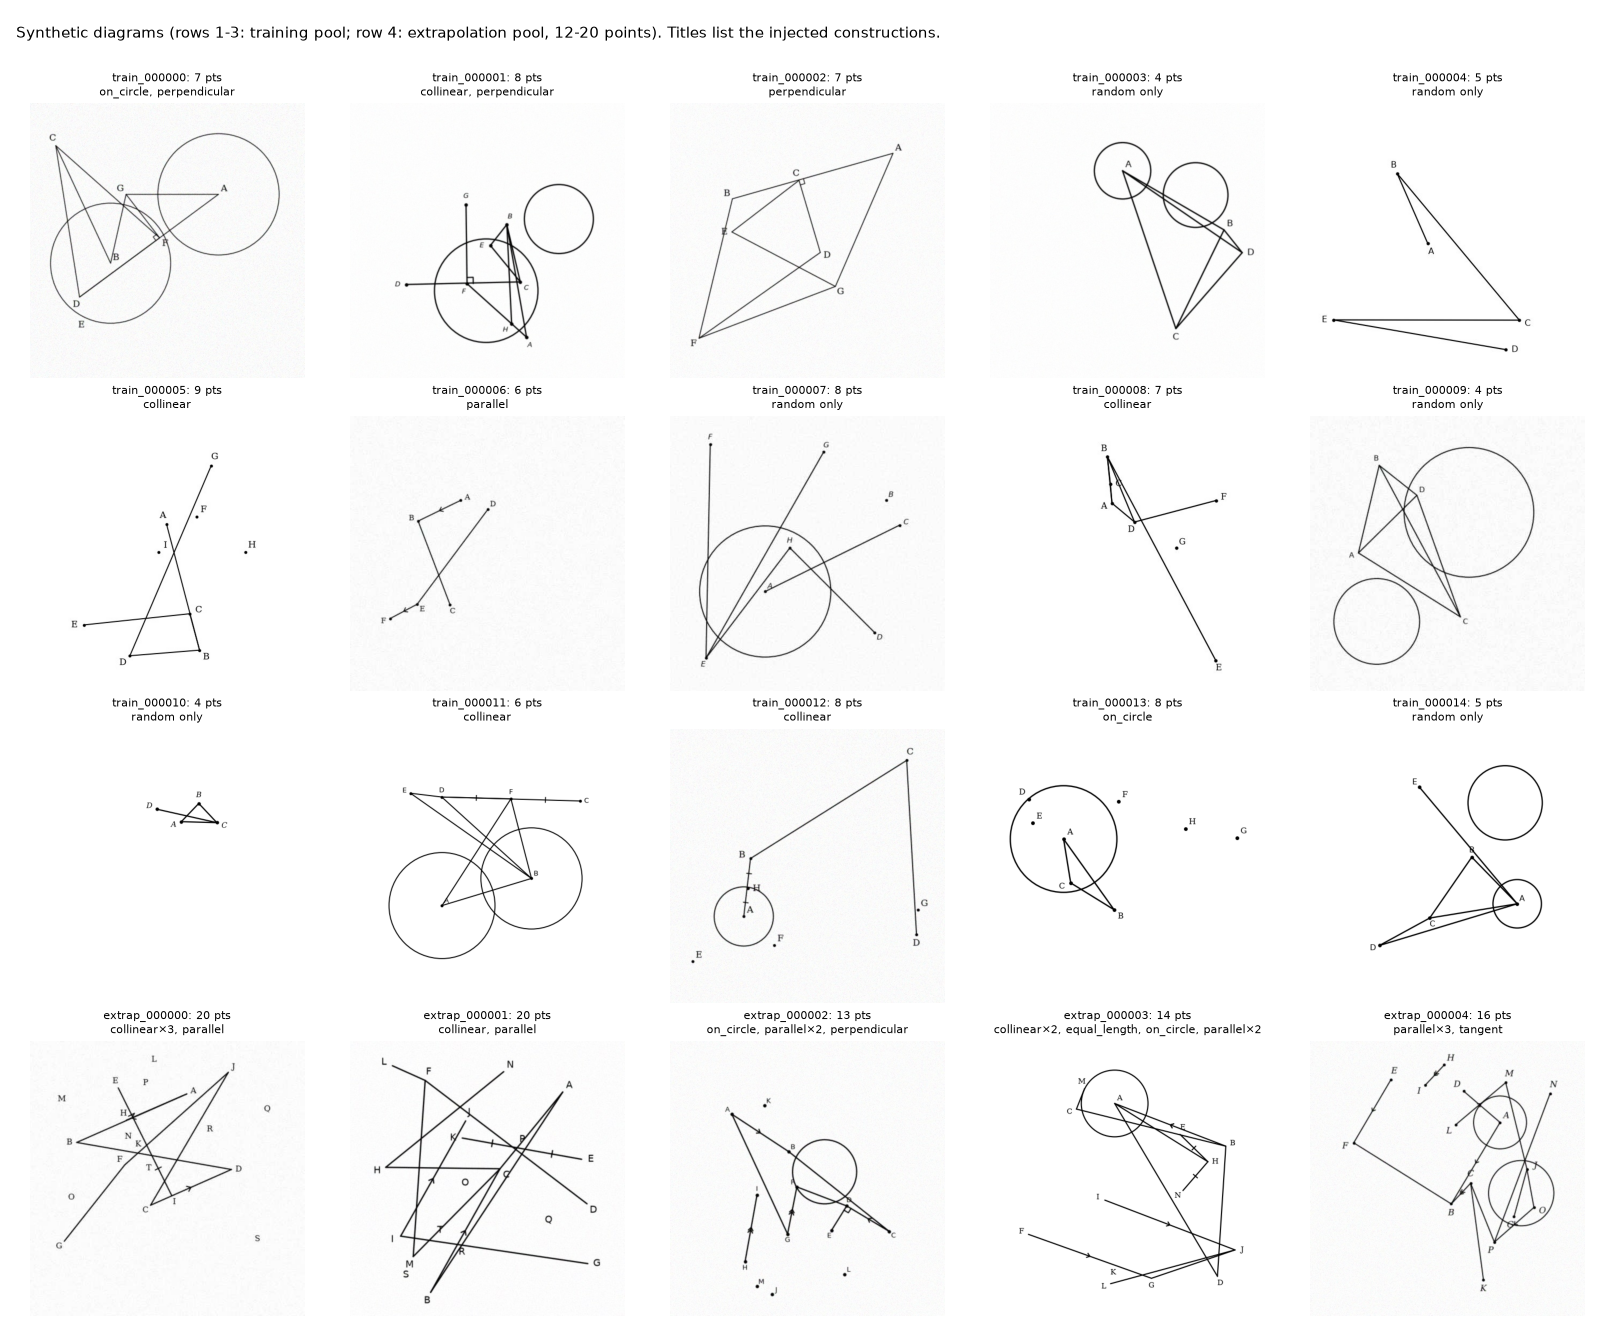
\includegraphics[width=\textwidth]{synthetic_examples}
  \caption{Synthetic diagrams from the training pool, with the injected relations drawn as marks and the rendering style varied.}
  \label{fig:synthetic}
\end{figure}
